\documentclass[12pt,a4paper,openright]{article}
\usepackage[utf8]{inputenc}
\usepackage[spanish]{babel}
\usepackage{amsmath}
\usepackage{amsfonts}
\usepackage{amssymb}
\usepackage{subfigure}
\usepackage{enumerate}
\usepackage{graphicx}
\usepackage[left=2cm,right=2cm,top=2cm,bottom=2cm]{geometry}
\author{Jorge Benz Olguín Aguilar}
\title{Actividad 5}

\begin{document}
\maketitle

\section*{Introducción}

En lecciones anteriores se ha descrito el concepto de diseño descendente; esta técnica permite desarrollar
algoritmos que resuelvan un problema mediante un proceso de refinamiento progresivo, descomponiendo el problema
original en subproblemas menores hasta obtener una granularidad suficientemente fina que permita resolver cada
subproblema mediante un algoritmo sencillo.
Generalmente, por cada nivel del diseño descendente se desarrollo un pseudocódigo de alto nivel que hace
uso de acciones no primitivas; si se detecta que alguna de estas acciones no primitivas aparece más de una vez es
posible nombrarla y utilizarla de forma repetida. Tales acciones con nombre se denominan subprogramas y pueden ser,
a su vez, funciones y subrutinas \\

La utilización de subprogramas proporciona múltiples ventajas:
\begin{itemize}
\item Facilitan la modularidad y estructuración de los algoritmos.
\item Facilitan la lectura e inteligibilidad de los algoritmos.
\item Permiten una economización del esfuerzo del programador al poder escribir código reutilizable en muchas
partes de un mismo algoritmo.
\item Facilitan la depuración y mantenimiento de los programas.
\end{itemize}


\subsection*{Funciones}

Las funciones son subrutinas que pueden tener o no argumentos pero que siempre devuelven un valor de
retorno. Así pues, las invocaciones a funciones son expresiones de un tipo determinado y deben emplearse igual que
cualquier expresión de su tipos; es decir, una llamada a función puede formar parte de una expresión aritmética, lógica o
de cadena en función de su tipo, puede constituir la parte derecha de una sentencia de asignación, aparecer en una
sentencia de salida o constituir un argumento para otro subprograma. Por otro lado, las llamadas a funciones nunca
pueden formar una sentencia aislada ni constituir la parte izquierda de una sentencia de asignación.

\subsection*{Subrutinas}

En muchas ocasiones puede interesarnos desarrollar un subprograma que no se vea afectado por las
limitaciones de las funciones; es decir, puede interesarnos un subprograma que sea capaz de “retornar” varios valores o
ninguno. Para esos casos existen las denominadas subrutinas o procedimientos; las subrutinas son subprogramas que
no devuelven ningún resultado, por tanto no tienen tipo, y en los que es “lícito” emplear los efectos laterales antes
mencionados para permitir al programa principal obtener varios valores “resultantes” de la ejecución del subprograma.
Las subrutinas se diferencian de las funciones fundamentalmente en la sintaxis de la definición y en la forma de
invocarlos; dado que no tienen tipo alguno las subrutinas no pueden formar parte de expresiones ni aparecer en la parte
derecha de una sentencia de asignación, deben aparecer única y exclusivamente en una sentencia de llamada a
procedimiento.




\section*{Actividades a realizar}


Nos interesa utilzar el concepto de funciones en Fortran, para desarrollar una función "Taylor", a la que le demos un par de valores de una función y nos regrese el valor de la Serie de Taylor para un punto.\\

Escriba una función de Taylor en Fortran, que utilice la primera y segunda derivada, por lo que requiere entonces de conocer los valores de una función en $f(x-h)$, $f(x)$  y $f(x+h)$. \\

Utilizando las aproximaciones de diferenciación numérica para la primera y segunda derivada, calcule el error E(x) como función de x, de aproximar con los primeros 3 términos a una función f(x), para los siguientes casos. \\

\begin{enumerate}

\item f(x) = sin(x), alrededor de a=0.
\item f(x) = cos(x), alrededor de a=0.
\item f(x) = tan(x), alrededor de a=0.
\item f(x) = exp(x), alrededor de a=0.

\end{enumerate}
 
 
 Grafique las funciones error $E(x)= f(x) - Taylor(x,a)$, como función de x para cada uno de los casos. \\
 
\begin{large}
 El codigo fuente del programa utilizado
 \end{large} 
 
\begin{verbatim}

program taylorprogram
  
  IMPLICIT NONE

  INTERFACE
     
     FUNCTION SerieTaylor(f_0,f_1,f_2,h)
       REAL :: SerieTaylor
       REAL, INTENT(IN) :: f_0, f_1, f_2, h
     END FUNCTION SerieTaylor
    END INTERFACE
 
  REAL :: x_0, x_1, x_2, h, suma, F
  INTEGER :: i, npts, icaso  
  write(*,*) "Ingresa el numero correspondiente para el caso deseado caso seno: 1 ,coseno: 2 ,tangente: 3 ,exponencial: 4."
  read(*,*) icaso
  write(*,*) icaso  
  npts=21
    
     write(*,*) "Serie de Taylor del Caso Seleccionado Anteriormente"
     h=0.1
   
     do i=1, npts
        x_0=float(i-1)*h
        x_1=float(i)*h
        x_2=float(i+1)*h
       suma =SerieTaylor(F(x_0,icaso), F(x_1,icaso), F(x_2,icaso), h)
     
       write(*,*) i, suma, F(x_1,icaso), (suma-F(x_1,icaso))               
       open(unit=12, file='Error.dat')
       write(12,*)i, suma-F(x_1,icaso)      
     end do
    close(12)
  
   END PROGRAM taylorprogram   
   
   FUNCTION SerieTaylor(f_0,f_1,f_2,h)
    
     IMPLICIT NONE
     REAL :: SerieTaylor
     REAL, INTENT(IN) :: f_0, f_1, f_2, h
     SerieTaylor=f_1+((f_2-f_0)/(2*h))*h+((f_2-2*f_1+f_0)/(2*h*h))*h*h
    
     END FUNCTION SerieTaylor
    
     FUNCTION F(x,icaso)
      
       IMPLICIT NONE
       REAL :: F
       REAL, INTENT(IN) ::  x
       INTEGER, INTENT(IN) :: icaso
       if (icaso.EQ.1) then
          F=sin(x)
       end if      
  
       if (icaso.EQ.2) then
          F=cos(x)
       end if
       if (icaso.EQ.3) then
          F=tan(x)
       end if
       if (icaso.EQ.4) then
          F=exp(x)
       end if  
     
     END FUNCTION F
     

\end{verbatim} 

Las gráficas obtenidas apartir del Codigo. Las graficas muestran el error obtenido entre la medición y la apŕoximación.\\

\begin{figure}[htb]
\centering
\subfigure[Error seno]{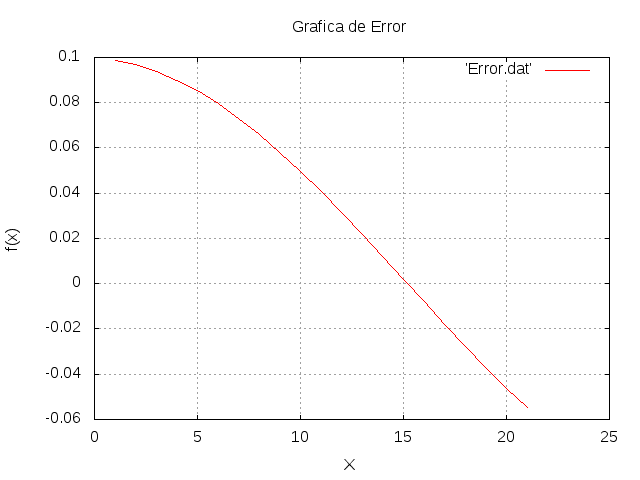
\includegraphics[scale=0.4]{Error1.png}  } \hspace{10mm}
\subfigure[Error Coseno]{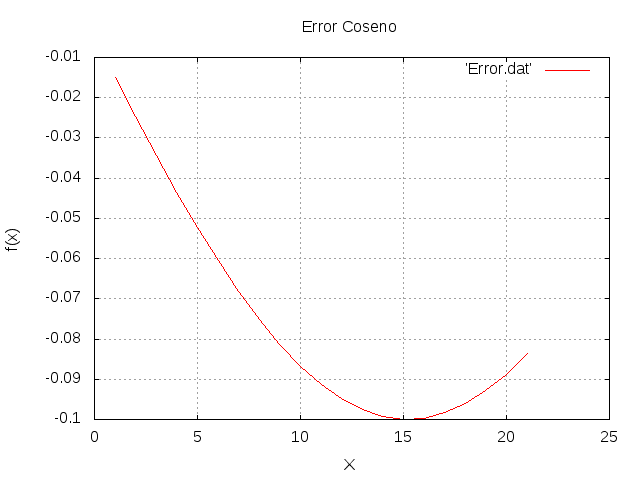
\includegraphics[scale=0.4]{Error2.png}}
\subfigure[Error Tangente]{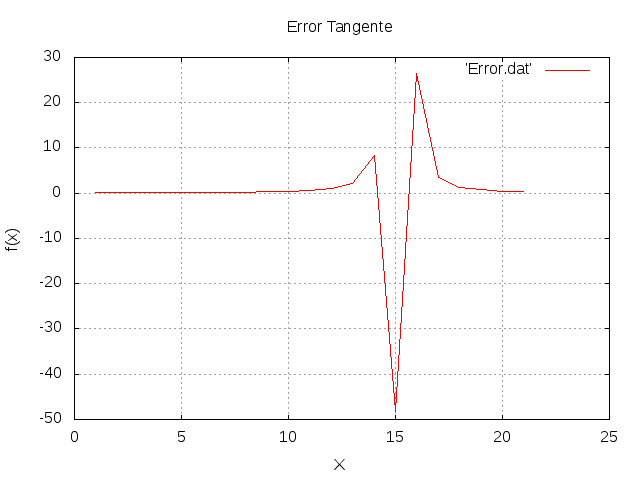
\includegraphics[scale=0.4]{Error3.png}} \hspace{10mm} 
\subfigure[Error Exponencial]{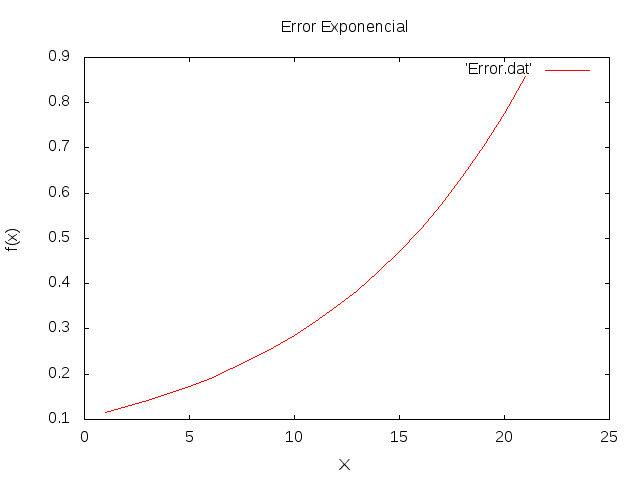
\includegraphics[scale=0.4]{Error4.png}} 
\caption{Errores de las mediciones contra los valores reales} 
\end{figure}




\end{document}